% textidote: ignore begin
\chapter{Method}\label{ch:method}
% textidote: ignore end


\section{How can we help solve this problem?}\label{sec:how-can-we-help-solve-this-problem?}

The expected outcome from making this service is to cause help people travel in their preferred way.
Making this program would also allow users to plan their journey days before, which would improve traffic flow
overall and quality of life for the consumers.

We gather data from ``rejseplanens'' API such that we can request data about the public transport in Denmark.
We further investigate the environmental factors where we investigate how much \unit{CO_{2}} emission
different car types and public transport types causes per kilometer.

We research how much \unit{CO_{2}} emission different types of cars cause and set them to an average for
the program parameters to make it simpler to calculate routes with less \unit{CO_{2}} emission.
The same goes for public transport.
We research how much \unit{CO_{2}} emission trains, buses and metros emit.

We allow users to make different priorities such as the time of arrival, cost, environmental impact and comfort.
Furthermore, a filter is added where the user is able to set their own priorities.

The user interface (UI) is supposed to be user-friendly for all consumers, such that it can be used effectively by all
consumers.
The UI we are using for this project is the terminal, which is text-based.
The reason for the choice of our UI is limited by the projects restrictions in which we were recommended to make a
terminal UI instead of another more user-friendly graphical UI\@.

\section{Solution stack}\label{sec:solution-stack}

In the following section, we will take a closer look at the solution stack that the development team has chosen to use
to create the software that will constitute the problem solution.

\subsection{Development team}\label{subsec:development-team}

The development team consisted of seven young computer science students with different levels of previous development
experience.

\subsection{Basic requirements}\label{subsec:basic-requirements}

Before the development team began the development process, a wide variety of basic technological and workflow-related
requirements and constraints were discussed.

The team understood very quickly that high productivity and development efficiency were one of the top priorities for
the task at hand, due to the relatively short deadline, development team size and the complexity of the software's
logic.

Other constraints were identified as well, such as the fact that while every member of the development team had
different levels of experience with different programming languages and technologies, everyone was familiar with the
C programming language.

Finally, coming from a wide range of backgrounds and having different preferences, the individual members of the team
wanted to be able to make individual choices regarding their development setups, while still maintaining project-level
coherency.
Examples of such individual preferences included which development operating system each member would work on (such as
Windows 11, macOS, various Linux distributions, and also Windows Subsystem for Linux (WSL)).
Additionally, individual preferences extended to choices regarding what code editor or intelligent development
environment (IDE) the member would use.
And finally, another constraint dictated by personal preferences was what tools were available for the chosen
development platform, such as compilers, linters, etc.

Those three basic realizations largely dictated all the other choices of technologies, workflows and other development
tools.

\subsection{Version control}\label{subsec:version-control}

When dealing with a software project of this size and complexity, combined with a development team of this size, it is
crucial to be able to collaborate remotely over the internet.
Also, it is paramount that the team is able to trace incremental changes in the software source code.
This is where version control and version control systems come into play.

\subsubsection{Version control system}

For this project, the team selected the \lstinline{git} version control system, which is modern, efficient and
relatively easy to use.
The usage of \lstinline{git} allowed each team member to develop incremental features and changes on their own
development machine and then combine the changes on the \lstinline{main} version control branch.
To further ease the process and make individual development fully independent, a server was needed to which the
individual members' contributions could be uploaded.
For this task, \href{https://github.com/}{GitHub} was chosen, and a public code repository was created using the private
GitHub account of one of the team members.
The repository can be found here: \href{https://github.com/audio-engineer/aau-p1-software}{aau-p1-software}.

\subsubsection{Branching model}

Modern version control using \lstinline{git} relies on the idea of \textit{branching}.
\textit{Branches} consist of a series of \textit{commits}, which are snapshots of the source code taken at arbitrary
times by the developers while working on their development machines.
The team decided that the easiest approach to branching would be a model based heavily on \textit{trunk-based
development}~\cite{trunk-based}, which is a simple model where all changes from individual branches are merged directly
into the project's \lstinline{main} branch without additional branching complexity.
Additionally, to keep the development routines as simple and efficient as possible, it was decided that each developer
would have their own branch on which they would continuously commit their individual contributions.
Those branches were then continuously uploaded (\textit{pushed} in \lstinline{git} terminology) to GitHub, where they
were merged into the \lstinline{main} branch.
Each time after a merge was completed, the contributor in question's branch was reset to match the \lstinline{main}
branch, upon which the development cycle was resumed.

We will take a closer look at how it was implemented practically in the Section~\ref{sec:workflows-and-routines}.

\subsection{Development systems and tools}\label{subsec:development-systems-and-tools}

As previously mentioned, the team's personal development setup preferences varied, not least in the choice of code
editor or IDE, and development machine operating system.
Simultaneously, it was determined that to maximize efficiency, some project configurations and other related settings
would have to be shared across development machines and operating systems.
This was deemed necessary to prevent that each developer would have to set up their local development environment
from scratch.
To mitigate this issue, some sort of configuration sharing was necessary to be introduced into the development flow.
Luckily, a majority of the developers were already familiar with the IDE vendor JetBrains' products, which offer great
support for shared configurations~\cite{shared-config}.
Therefore, a shared configuration was added to the source code repository, which was then read by each developer's
IDE upon opening the project.
Examples of configurations that were shared include code indentation and bracket placement style, unit test runner
configuration, text encoding, required IDE plugins and code linting settings.

\subsection{Programming languages}\label{subsec:programming-languages}

As was mentioned in the Section~\ref{subsec:basic-requirements}, the C programming language was the single
programming language that all developers in the team were familiar with, which is one of the primary reasons why it was
chosen as the development language.

Another reason was the flexibility that C offers: It can be developed and compiled for a wide range of target systems.
In other words, C offers cross-platform compatibility both from development and distribution perspectives.

It was also decided early on that the solution application would be a console application, and C also has the advantage
that it is an excellent language for console application development.

Finally, C has been on the market for many decades and is a very well-established language with exceptional tooling and
availability of libraries, compilers, IDEs, and frameworks that support it, making it a good choice for many tasks.

But while C made up the majority of the source code, it also turned out to be necessary to introduce C++ into the
project, due to the usage of the \textit{GoogleTest} unit testing library.
GoogleTest is originally built for usage with C++, but can easily be adopted to be used with purely C-based projects,
only requiring slight modifications to how the project is built and how the tests are written.
Also, luckily GoogleTest is almost exclusively built on macros, which made writing tests a lot easier for the team,
since only very little or almost no C++ syntax had to be learned.
This will be further discussed in the Section~\ref{subsec:testing}.

\subsection{Integrations}\label{subsec:integrations}

In the following section we will take a closer look at the integrations that will help us create the software.
We will be taking a further look into what an REST-API is, and we would also be looking into how Rejseplanens API works
and how we are going to use it for this project.

\subsubsection{\uppercase{Rest API}}\label{subsubsec:rest-api}

To understand what a REST API is we will look further into what a NON-REST-API is and what it does.
It will all be explained shortly what an API is.

\subsubsection{What is an API}\label{subsubsec:what-is-an-api}

Application Programming Interface (API), is a way for two or more programs to communicate with each other.
It is a type of interface for software as it can service other pieces of software.
An API is often made up of different parts which can act as a tool for the programmer, when a programmer is using the
API they can make \textit{calls} to different parts of the API\@.
The \textit{calls} that make up the API are also known as \textit{methods, requests or endpoints}~\cite{APIwiki}.

The purpose of an API is that it simplifies programming by abstracting the implementation and only exposing the objects
or actions the developer needs.
An API makes it so that a developer can press a button in a program that does something like replacing files one place
to another without the developer needing to understand the operations occurring behind the scenes.

\subsubsection{What is a REST API}\label{subsubsec:what-is-a-rest-api}

A REST API is an API that goes by the design of REST also known as \textit{representational state transfer}
architectural style.
It is called a REST API because it uses a certain design compared to other APIs where some use different frameworks
such as SOAP where its data is strictly XML-format and where REST is more flexible being able to support a larger
framework for data transfers as REST supports different formats, including \textit{XML, HTML, plain text, JSON... and
more}~\cite{IBMrestapi}.

REST APIs communicate via HTTP requests to perform simple database functions such as \textit{creating, reading,
    updating and deleting records}~\cite{IBMrestapi}, an example could be that a REST API would want to use a GET
request to retrieve data and a POST request to create data, a PUT request to update the data and a DELETE request to
delete data.

\subsubsection{Key principles and characteristics of a RESTful API}
\label{subsubsec:key-principles-and-characteristics-of-a-restful-api}
\begin{itemize}
    \item \textbf{Staleness}: Each request made from a client to a server must contain all the information needed to
    understand and process that request.
    The server should not store any information about the client's state between requests.
    This enhances scalability and simplifies server implementation.
    \item \textbf{CRUD Operations}: RESTful APIs use standard HTTP methods (GET, POST, PUT, DELETE) to perform CRUD
    operations on resources so that would be (Create, Read, Update, Delete).
    Each HTTP method corresponds to a specific action on the resource.
    \begin{itemize}
        \item \textbf{GET}: Retrieves a representation of the resource
        \item \textbf{POST}: Creates a new resource
        \item \textbf{PUT}: Updates an already existing resource
        \item \textbf{DELETE}: Removes an existing resource
    \end{itemize}
    \item \textbf{Representation}: The resources are represented in a format, such as JSON or XML.
    The client and server has to agree on which format the data needs to be in during the communication.
    JSON and XML is often preferred because it can be read by a human and is therefore easier to navigate.
\end{itemize}
% textidote: ignore begin

\subsection{Rejseplanens API}\label{subsec:rejseplanens-api}
% textidote: ignore end

\subsection{Build system}\label{subsec:build-system}

One of the disadvantages of C, though, is that it requires a solid and substantial ecosystem of build tools and
compilers around the C source code to be able to build the distribution-ready application.
One approach would be to let each developer set up their own build system to be able to compile the source code on their
local development environment, and then later decide on a \textit{master} compilation machine where the distribution
version would be compiled.
But the development team chose an approach where the build configuration was built into the source code itself, making
it easy to share it across local development environments.
This also allowed each developer to build the software using the same build parameters.

The primary tool picked to solve this task was CMake, which is a build automation tool that generates build
configuration files based on a common project configuration.

CMake also has the advantage that it can prepare the compilation machine for compilation by searching for compilation
dependencies aka ``dependencies of dependencies'' without which the compilation would fail.
For this purpose, the team made use of the \lstinline{pkg-config} CMake integration.
\lstinline{Pkg-config} is a tool that searches the compilation machine exactly for those prerequisite dependencies to
make sure that all direct dependencies and if they are not found, the compilation is aborted.
If they are, on the other hand, found, the application compilation is resumed and completed.

Furthermore, CMake also allows for the addition and management of external software dependencies such as libraries
and frameworks, which will be discussed in the Section~\ref{subsec:libraries-and-frameworks}.

\subsection{Libraries and frameworks}\label{subsec:libraries-and-frameworks}

% TODO Add more content to this subsection
// cURL, cJSON, OpenSSL

Very early on in the solution architecture design process, it became clear to the team that external libraries and
frameworks would have to be used.
The two primary reasons for this were the fact that C, the chosen programming language for this project, does not
include features like making HTTP calls, nor does it have support for the JSON data format.
Those two features are crucial when designing software that talks to and consumes data from REST APIs, as discussed
in the Section~\ref{subsubsec:rest-api}.
The team therefore decided to introduce two external libraries that would provide additional functions that could
deal with HTTP and JSON to the C language, namely \lstinline{cURL} and \lstinline{cJSON} respectively.

How the external libraries were linked to and compiled with the software's source library can be seen in
\ref{fig:figure10}.

% TODO Insert CMake dependency, compilation and linkage flowcharts

\begin{figure}
    \centering
    \caption{The software's dependencies.}
    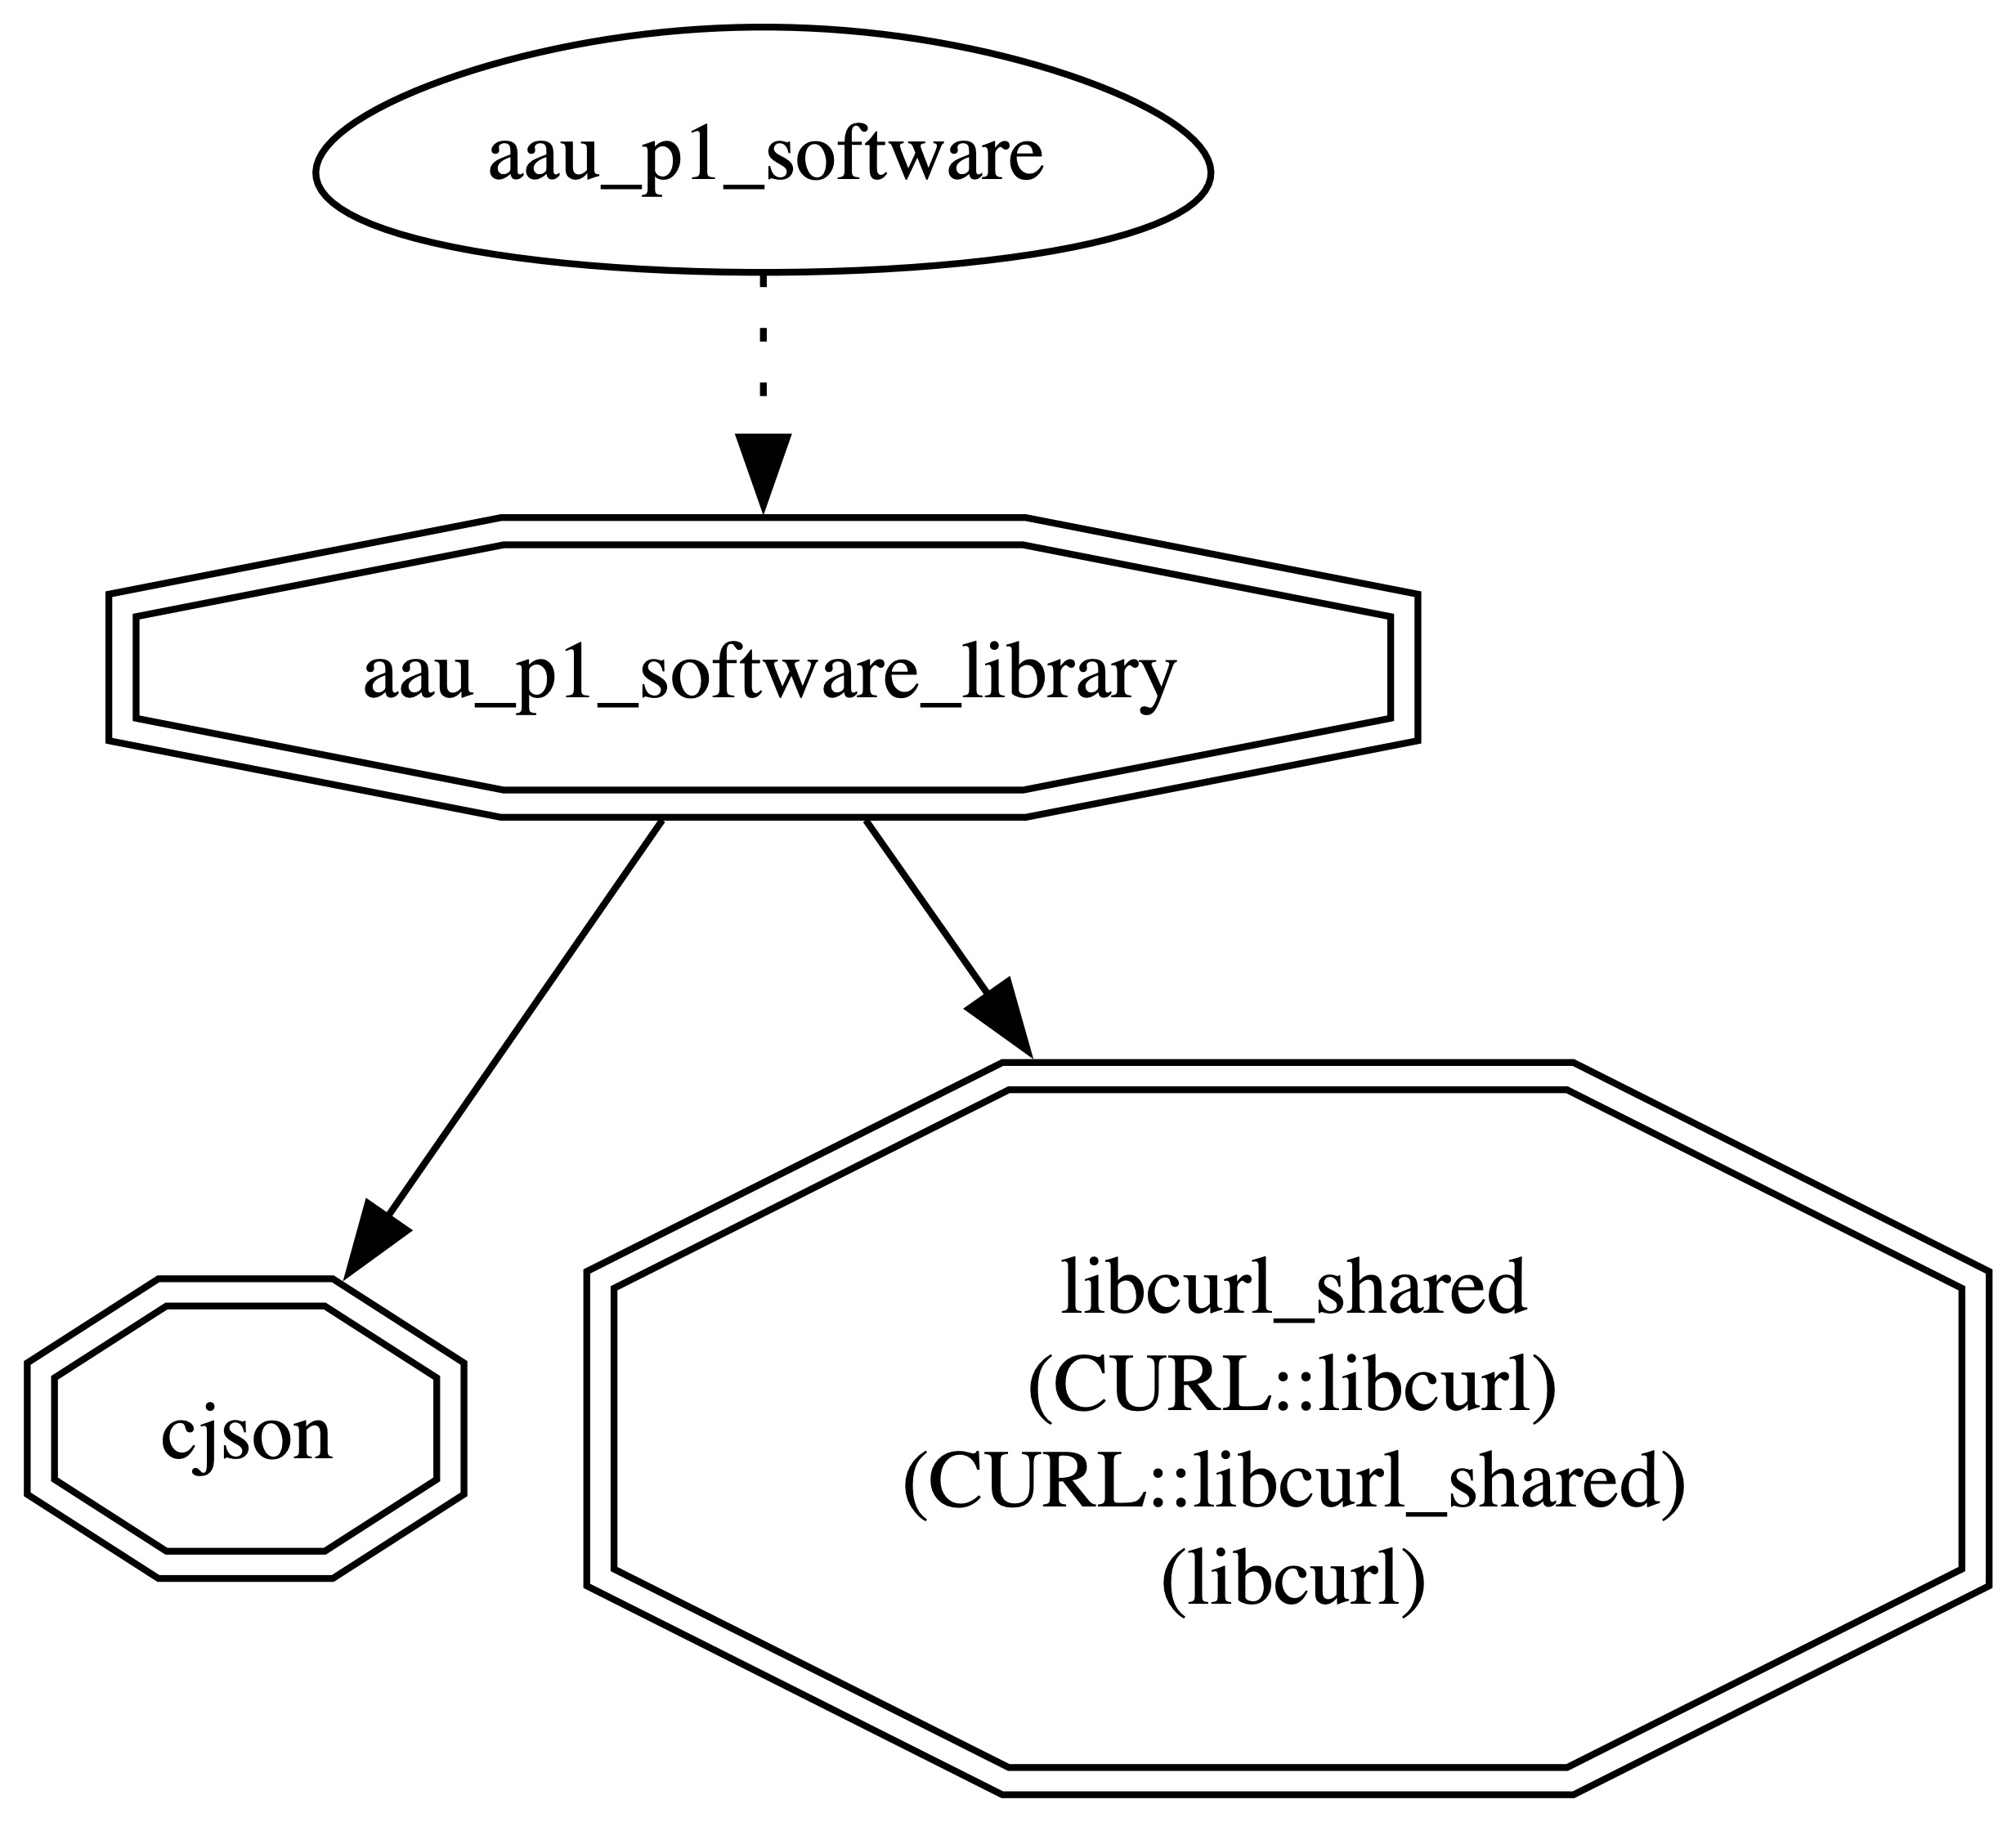
\includegraphics[width=0.5\textwidth]{aau-p1-software}
    \label{fig:figure10}
\end{figure}

\subsection{Code style and quality}\label{subsec:code-style-and-quality}

When working on larger scale software projects where more than one developer is involved, it is also crucial to keep the
source code readable, maintainable and coherent to be able to easily develop and refactor it later.
For this reason, the team decided to use a common code style and use tools to ensure that this style was complied with.
As a baseline, it was decided that the Google C++ Style Guide~\cite{google-style} would be used for basic stylistic
features such as function, data and file naming conventions, an indentation width of two spaces, bracket placement, etc.
While the Google C++ Style Guide is, as the name suggests, made for C++ projects, it can easily be adopted for usage
with C projects by simply adhering only to the style guidelines that regard features that both C++ and C share.

To assist the developer team with adhering to those guidelines, the \textit{Clang-Format}~\cite{clang-format} and
\textit{Clang-Tidy}~\cite{clang-tidy} tools provided by the \textit{Clang} compiler were used to automatically lint
the code for breaches of style.
This process was made even easier due to the seamless integration of these tools into the JetBrains CLion IDE that was
used by a majority of developers, which made it possible to lint the source code while writing it.

// ClangFormat, ClangTidy, EditorConfig, Google C++ Style Guide, pull requests and code reviews.

We will take a closer look at how it was implemented practically in the next Section~\ref{sec:workflows-and-routines}.

\subsection{Testing}\label{subsec:testing}

As mentioned in the Section~\ref{subsec:programming-languages}, the teams uses GoogleTest to evaluate functions and
methods in the code. GoogleTest is a framework for writing C++ tests on a variety of platforms (Linux, Windows, Mac OS
X, etc.)~\cite{googletest}.
GoogleTest is a framework that is used to test C++ code, but it can also be used to test C code.
The reason why the team chose to use GoogleTest is because of the size of the team and the complexity of the project.
GoogleTest allows for the team to test functions and methods in the code, without including them in main code.
It does this by creating a separate file for the tests, which is then compiled and run separately from the main code.
This allows for the team to work on individual parts of the code, without having to worry about interfering with each
other.


% textidote: ignore begin

\subsection{CI/CD}\label{subsec:ci/cd}

% TODO Add more content to this subsection
// GitHub Workflows/Actions

\subsection{Target systems}\label{subsec:target-systems}
% textidote: ignore end

% TODO Add more content to this subsection
// Cross-platform (Windows, macOS, Linux)

\section{Workflows and routines}\label{sec:workflows-and-routines}

In this section, we will discuss the development team's routines and workflows to gain a better understanding of how
the development process looked like.
The team's workflow for both the program and the report consisted of collaboration, communication, and version control.
Microsoft Teams was used for communication, Trello was used to assign tasks, and GitHub was used for the development of
the project.
Discussions were held in person and Microsoft Teams.
After the discussions, the team would create Trello cards for the task and assign them to individual members.
The GitHub repository has separate branch for each member of the team.
The team would work on their personal branch and then create a Pull Request with the purpose to merge the changes to the
main branch.
The Pull Request would then have to be reviewed by at least 2 other members before it could be merged.
After the merge, the person responsible for the changes will reset their branch and reuse it for the next task.
This workflow was used for both the program and the report.

GitHub has the added benefit of Actions, which is a CI/CD tool.
The team has set up different actions for the program and the report.
After a Commit on the program, GitHub will execute ClangTidy and ClangFormat workflows, that ensure that the code is
properly formatted and that there are no errors in the code.
The report has a workflow that will check for grammatical errors using TeXtidote and then compile the report into a PDF
file, which the team can then download and review.

The team had a weekly meeting with the supervisor, where the team would discuss the progress of the project.
Every meeting would start with a Code Review, where the team would go through the program and discuss the changes made
since the last meeting.
Occasionally, the team would also use the Scrum method to catch up on the progress of the project.
The team would discuss what they had done since the last meeting, what they were currently working on, and what they
would do next.

% TODO Add content to this section and remove `textidote: ignore begin/end`
% textidote: ignore begin
\section{Software project structure}\label{sec:software-project-structure}
% textidote: ignore end

It was decided to make use of an adopted version of the \textit{Pitchfork Layout}~\cite{pitchfork-layout}.

